% OUTPUT-SPACE ILLUSTRATION ONLY. For complete input-output window geometry,
% use io_trajectory_introduction.tex instead. This earlier text is superseded
% for the paper's intended trajectory-space example.
% Requires \usepackage{amsmath,amssymb,graphicx} in the main document.
% Copy cylinder_paper.pdf into the paper's figures/ folder, or adjust the path.

A simple example illustrates the geometric motivation for local representations.
Consider the controlled nonlinear system
\begin{equation}
\begin{aligned}
  \theta_{k+1} &= \theta_k+h\omega_k,\\
  z_{k+1} &= z_k+h(v_k+a\sin\theta_k),\\
  y_k &= (\cos\theta_k,\sin\theta_k,z_k)^{\mathsf T},
\end{aligned}
\label{eq:cylinder-example}
\end{equation}
where $(\omega_k,v_k)$ is the input, $h=0.12$, and $a=0.35$.
Its measured outputs satisfy $y_{1,k}^2+y_{2,k}^2=1$, so every rollout traces
a curve on a two-dimensional cylinder embedded in $\mathbb R^3$.
Figure~\ref{fig:cylinder-example} shows a family of rollouts sampling this
curved surface. As the angular position changes, the same angular input
produces motion in different directions in the measured output coordinates.
A single affine plane cannot represent the entire cylinder, whereas local
planes can approximate restricted neighborhoods. This example provides a
geometric motivation for grouping offline data according to the operating
condition and constructing local predictive representations. The cylinder
depicts the geometry of instantaneous outputs; the input-output trajectory
windows used for prediction generally occupy a higher-dimensional space.

\begin{figure}[t]
  \centering
  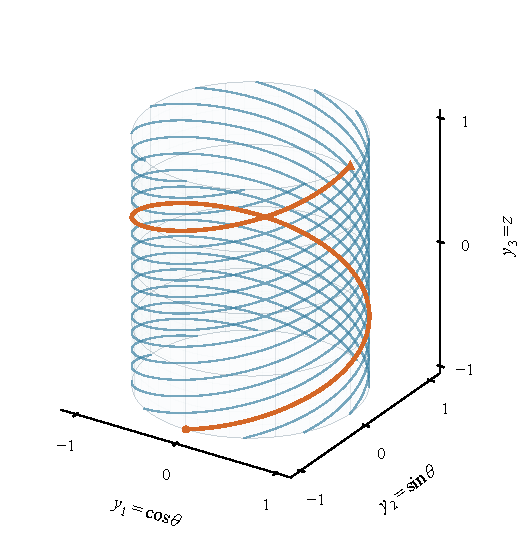
\includegraphics[width=\columnwidth]{figures/cylinder_paper.pdf}
  \caption{Curved output geometry of a simple nonlinear system.
  Twelve simulated rollouts, initialized at different angular positions,
  sample the invariant cylinder $y_1^2+y_2^2=1$ over $z\in[-1,1]$.
  The orange curve highlights one rollout; the circle and triangle mark
  its initial and final samples, respectively. Blue curves show the other
  rollouts, and the gray wireframe indicates the cylinder.
  Each rollout is a curve on the surface.}
  \label{fig:cylinder-example}
\end{figure}
